\section{$\text{LTL}_f\text{/LDL}_f$ Non-Markovian Rewards}
\label{section:nonmarkovianrewards}
Recently, non-Markovian reward decision processes (NMRDPs)
has attracted interest in the scientific community because of the possibility
of specifying them as MDPs with $\text{LTL}_f\text{/LDL}_f$ non-Markovian
rewards \cite{DBLP:journals/corr/abs-1807-06333}. In particular, it is possible
to model the problem with two separate representations of the world, one for
the agent (low-level) and one for the goal (expressed in terms of high-level
fluents).

This section presents the approach used in
\cite{DBLP:journals/corr/abs-1807-06333}, where an efficient method has been
developed in order to work with NMRDPs. The theory behind the main idea is
quickly described and an example on a theoretical Breakout environment is
discussed in order to be used in the following sections easily.

\subsection{Theoretical Background}
Before describing the problem, let's give a formal definition of NMRDP.
A non-Markovian reward decision process is a tuple $M = \langle S, A, \delta,
\bar{R} \rangle$, with $S$ finite set of states that can represent the
environment, $A$ is a finite set of actions that can be performed by an agent
in the environment, $\delta$ is a probability function modeling
the transition from a state to another when performing a certain action and
$\bar{R}: (S \times A)^* \rightarrow \mathbb{R}$ is a function from
finite state-action sequences (traces) to real-values that represents the
reward given by the environment when performing a certain state-action
sequence. Specifying a non-Markovian reward function explicitely is
difficult even when considering a finite number of traces. Luckily, the
$\text{LTL}_f\text{/LDL}_f$ formalism allows to specify $\bar{R}$
implicitely using a set of pairs $\{ (\phi_i, r_i) \}_{i=1}^m$ with
$\phi_i$ boolean
proposition over the components of the state vector and $r_i$ such that,
given a current trace $\pi = \langle s_, a_1, \dots, s_{n-1}, a_n \rangle$,
the agent receives at $s_n$ a reward $r_i$ if $\phi_i$ is satisfied by $\pi$,
hence:
\begin{equation}
    \bar{R}(\pi) =
        \begin{cases}
            r_i & \text{if } \pi \vDash \phi_i \\
            0 & \text{otherwise}
        \end{cases}
\end{equation}

Since the NMRDP rewards are based on traces, instead of state-action pairs,
typical learning algorithms like Q-learning or SARSA cannot be used.
Nevertheless, it has been shown \cite{DBLP:journals/corr/abs-1807-06333} that
for any NMRDP $M = \langle S, A, \delta, \{ (\phi_i, r_i) \}_{i=1}^m \rangle$
there exists an MDP $M' = \langle S', A', \delta' R' \rangle$ that is equivalent
to $M$. The idea behind the proof consists in starting from an initial
decision process $M_{ag}^{goal} = \langle S, A, R, \mathcal{L},
\delta_{ag}^g, \{ (\phi_i, r_i) \}_{i=1}^m \rangle$ with
$\text{LTL}_f\text{/LDL}_f$ goals (with $\mathcal{L}$ set of of configuration
of the high-level features needed for expressing $\phi_i$),
transform it into a NMRDP in order to
further transform it into a MDP where it is possible to execute learning
algorithms such as Q-learning. All the details are out of the scope of the
project and are discussed in \cite{DBLP:journals/corr/abs-1807-06333}. The
set of states $S$ is used to express low-level features of the agent.

The new MDP is extended by using automata needed to track the satisfiability
of a $\text{LTL}_f\text{/LDL}_f$ formulas, as explained in
\cite{DBLP:conf/aaai/2018}. Each formula is, hence, associated with an
automaton that accepts exactly the traces satisfying the formula itself.

Once the MDP has been determined it is possible to train a model that will
be able to manage non-Markovian rewards as well. Fig.
\ref{fig:rl-temporalgoals-pipeline} shows a pipeline of the
agent interacting with the world. In particular, a robot feature extractor
will analyze the state of the world $w$ in order to pass a representation $s$ to the
agent, a goal feature extractor will extract higher-level features of the world
$l$
that can be used to determine if a temporal goal has been achieved or not. In
positive case a reward $r$ is given to the agent. The evaluation $q$ of the formula
that specifies the temporal goals is given to the learning agent as well, in
order to construct an extended state of the MDP as specified by the theory above.
Each time the learning agent performs an action $a$, the environment changes
and it gives to the agent a reward $R$.
\begin{figure}
    \centering
    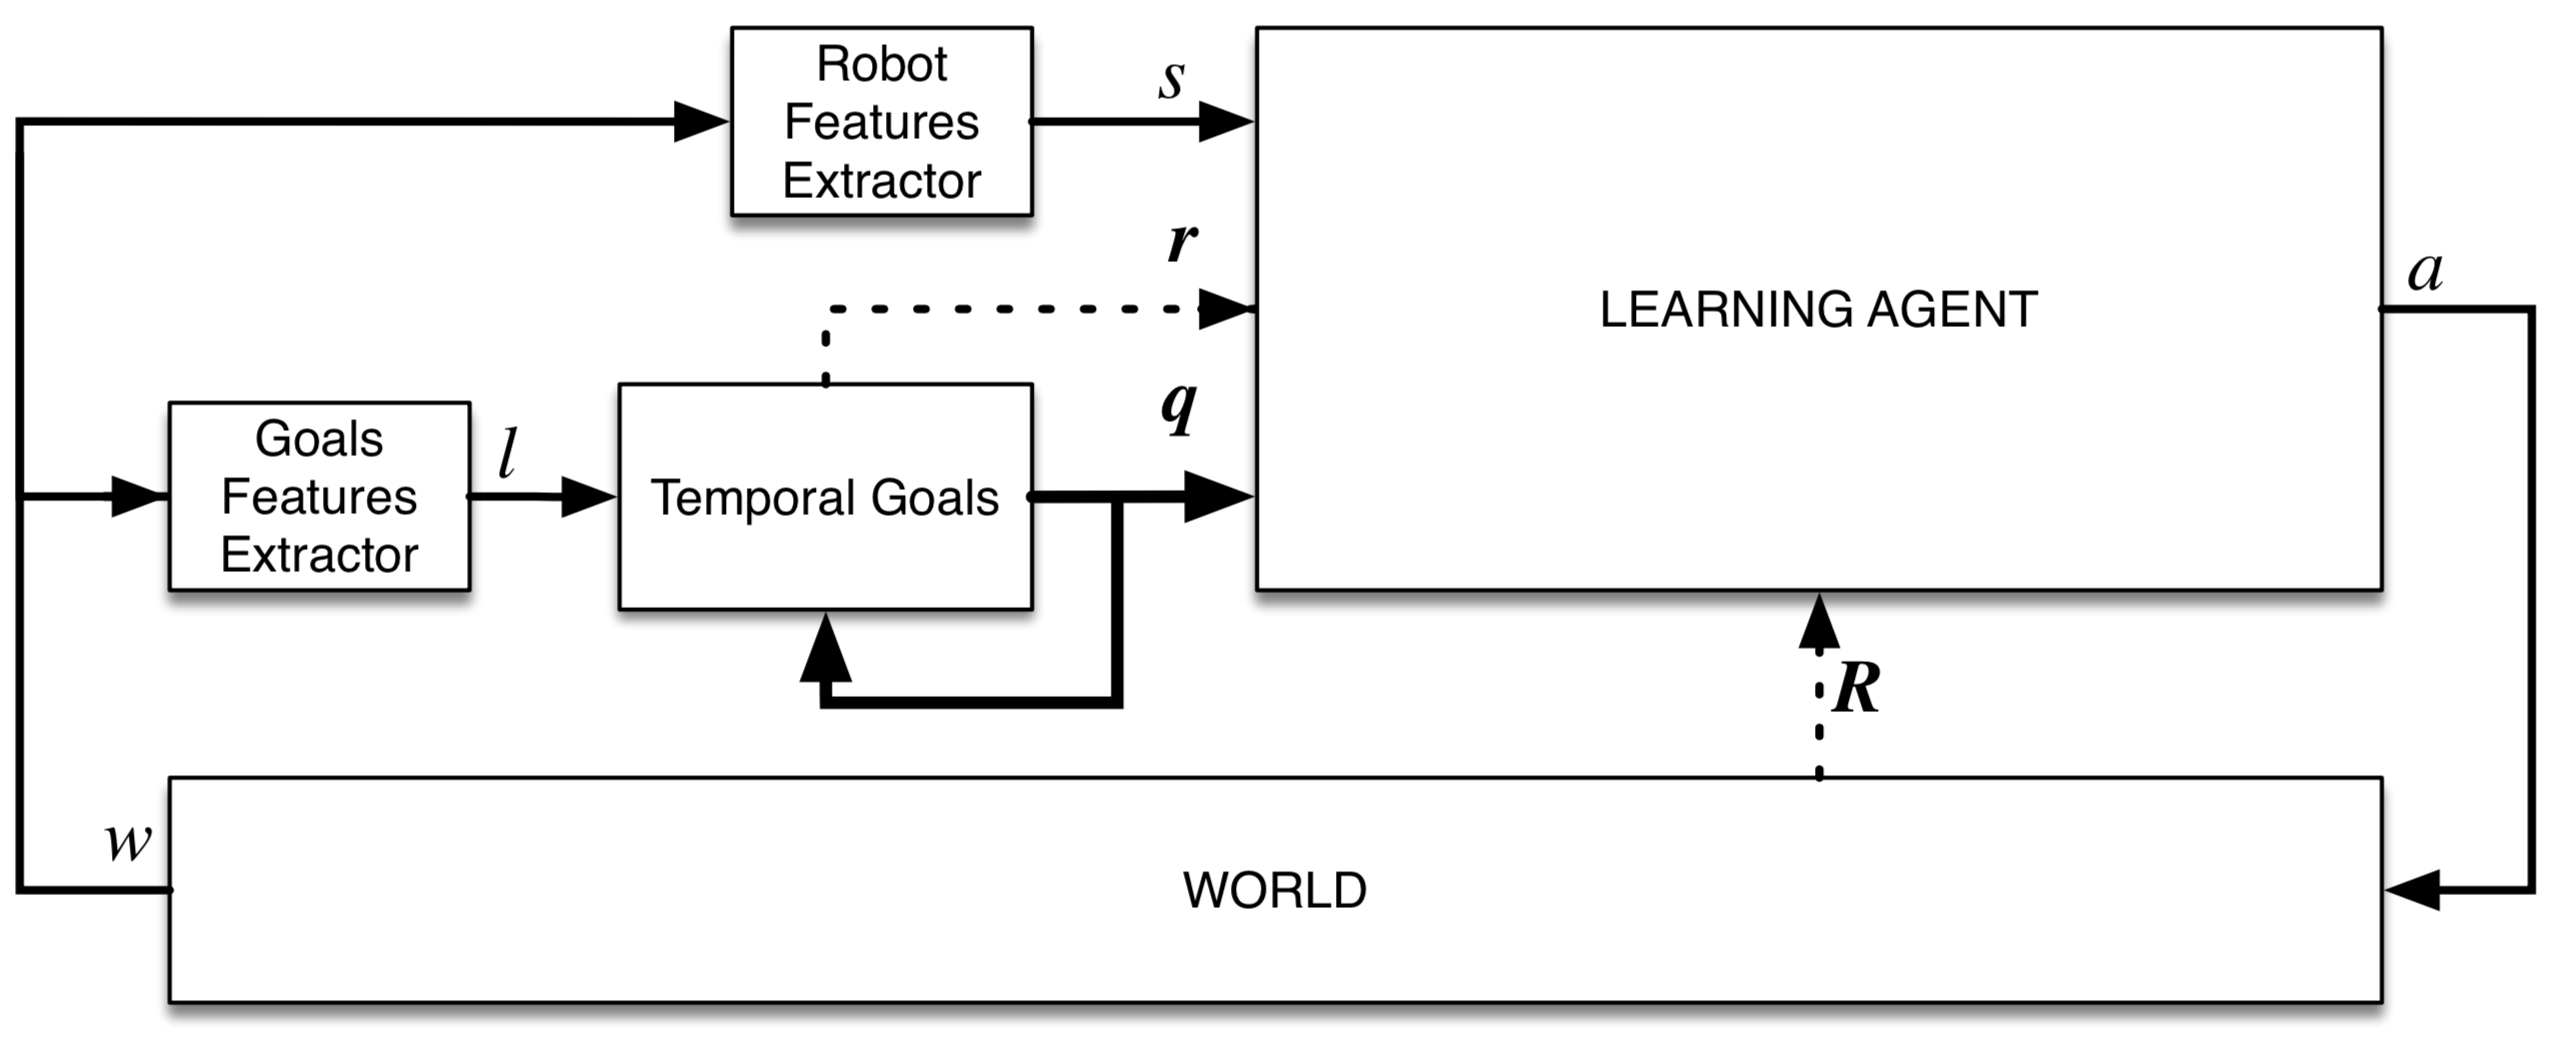
\includegraphics[width=0.85\textwidth]{images/rl-temporalgoals-pipeline.png}
    \caption{Pipeline describing how the agent is interacting with the
        world and how the robot features extractor and the goal features
        extractor are used in order to handle non-Markovian rewards.}
    \label{fig:rl-temporalgoals-pipeline}
\end{figure}

\subsection{Examples}
A typical example is breaking the bricks of a theoretical Breakout game in a
certain order. Let's consider a 3$\times$3 Breakout. A good idea is to use
$\text{LTL}_f\text{/LDL}_f$ goals to help the agent break to bricks from top
to bottom in order to make it create a hole on the left (or the right) and let
the ball do all the job without making any movements when it reaches the top
part of the environment. The idea is, hence, to help the agent learn
the most effective strategy, which should also decrease the training time.
Let's consider a formula that checks weather a row has been broken or not:
\begin{align}
\begin{split}
    \langle&(\neg\varphi_0 \land \neg\varphi_1 \land \neg\varphi_2)^*;
        (\varphi_0 \land \neg\varphi_1 \land \neg\varphi_2);
        (\varphi_0 \land \neg\varphi_1 \land \neg\varphi_2)^*;\\
        &(\varphi_0 \land \varphi_1 \land \neg\varphi_2);
        (\varphi_0 \land \varphi_1 \land \neg\varphi_2)*;
        (\varphi_0 \land \varphi_1 \land \varphi_2)\rangle tt
\end{split}
\end{align}

\noindent which, given $\varphi_0$ first row from the top broken,
$\varphi_1$ second row from the top broken and $\varphi_2$ third row from the
top broken, can be interpreted as:
\begin{itemize}
    \item $(\neg\varphi_0 \land \neg\varphi_1 \land \neg\varphi_2)^*$:
        initially, and for an indefinite amout of time, none of the rows have
        been broken;
    \item $(\varphi_0 \land \neg\varphi_1 \land \neg\varphi_2)$: then,
        the first row from the top has been broken but the remaining two
        are intact;
    \item $(\varphi_0 \land \neg\varphi_1 \land \neg\varphi_2)^*$: then,
        for an indefinite amount of time, the first row remains broken
        and the remaining two remain intact;
    \item $(\varphi_0 \land \varphi_1 \land \neg\varphi_2)$: then,
        the first two rows from the top have been broken and the remaining
        one at the bottom is intact;
    \item $(\varphi_0 \land \varphi_1 \land \neg\varphi_2)*$: then,
        for an indefinite amount of time, the first two rows from the top
        remain broken and the last one remain instact;
    \item $(\varphi_0 \land \varphi_1 \land \varphi_2)$: in the end,
        all the rows have been broken, hence, all the bricks have been broken.
\end{itemize}

In general, the formula $\langle\rho\rangle\phi$ states that, from the current step in
the trace, there exists an execution satifying $\rho$ such that in its last
step $\phi$ is satisfied. In the example above, at the end of the execution all
the rows have been broken.
